\section{RF codebook}
\label{sec:intro_q3}
The Random Forest vocabulary is a supervised visual vocabulary learning method that uses the leaf index as the quantization result. We trained the random forest after labeling 128-dimensional SIFT feature vectors by class number. For the testing data, each feature vector was assigned to the number of trees-leaves, resulting in a vector of dimensions equal to the number of trees. The mean of these vectors from image features was then used as the vector quantisation result.

\subsection{Optimizing hyperparameters}
We conducted experiments in a procedure similar to Section2 to find the optimal parameters for the Random Forest vocabulary. The results are shown in \cref{subsec:Q3-app1}. When $N$ (number of trees) = 8, $D$ (depth of trees) = 6, $\rho$ (number of attempts to split per node) = 10, we achieved sufficiently good performance with test accuracy of 60.67\% and the vocabulary size = 256.

\subsection{Comparison with Q2's result}
In \cref{fig:q3-fig4}, k-means vocabulary(Q2)'s overall accuracy and vector quantization time complexity is better than random forest codebook. Theoretical complexity is represented in \cref{subsec:Q3-app1}. However, since the vocabulary building and quantisation times for the random forest vocabulary that we obtained are less than 8 times those of k-means, we expect to get similar vector quantisation complexity when we implement parallelization for each tree.\\
In terms of training and testing error, the random forest codebook tends to extract relatively unsuitable features than k-means codebook, leading to underfitting. To demonstrate this, we performed quantization for vocabulary sizes of 64 and 256, and measured the value of (cosine similarity of inner-class vectors) divided by (cosine similarity of between-class vectors). As shown in \cref{table:q3-1} and \cref{table:q3-2}, the k-means codebook result in higher values at same vocabulary size, indicating that it performed better feature extraction for classification. The reason for this, as shown in the \cref{subsec:Q3-app2}, is that our random forest codebook has relatively less sparse quantization results compared to k-means. In k-means, a single SIFT feature contributes to a single histogram bin while in the random forest approach, one feature descriptor contributes to the (number of trees)-histogram bins. Additionally, since the random forest classification model which follows after vector quantization is sufficiently strong, the benefit of performing supervised vocabulary building is not significant.

\begin{figure}
	\centering
	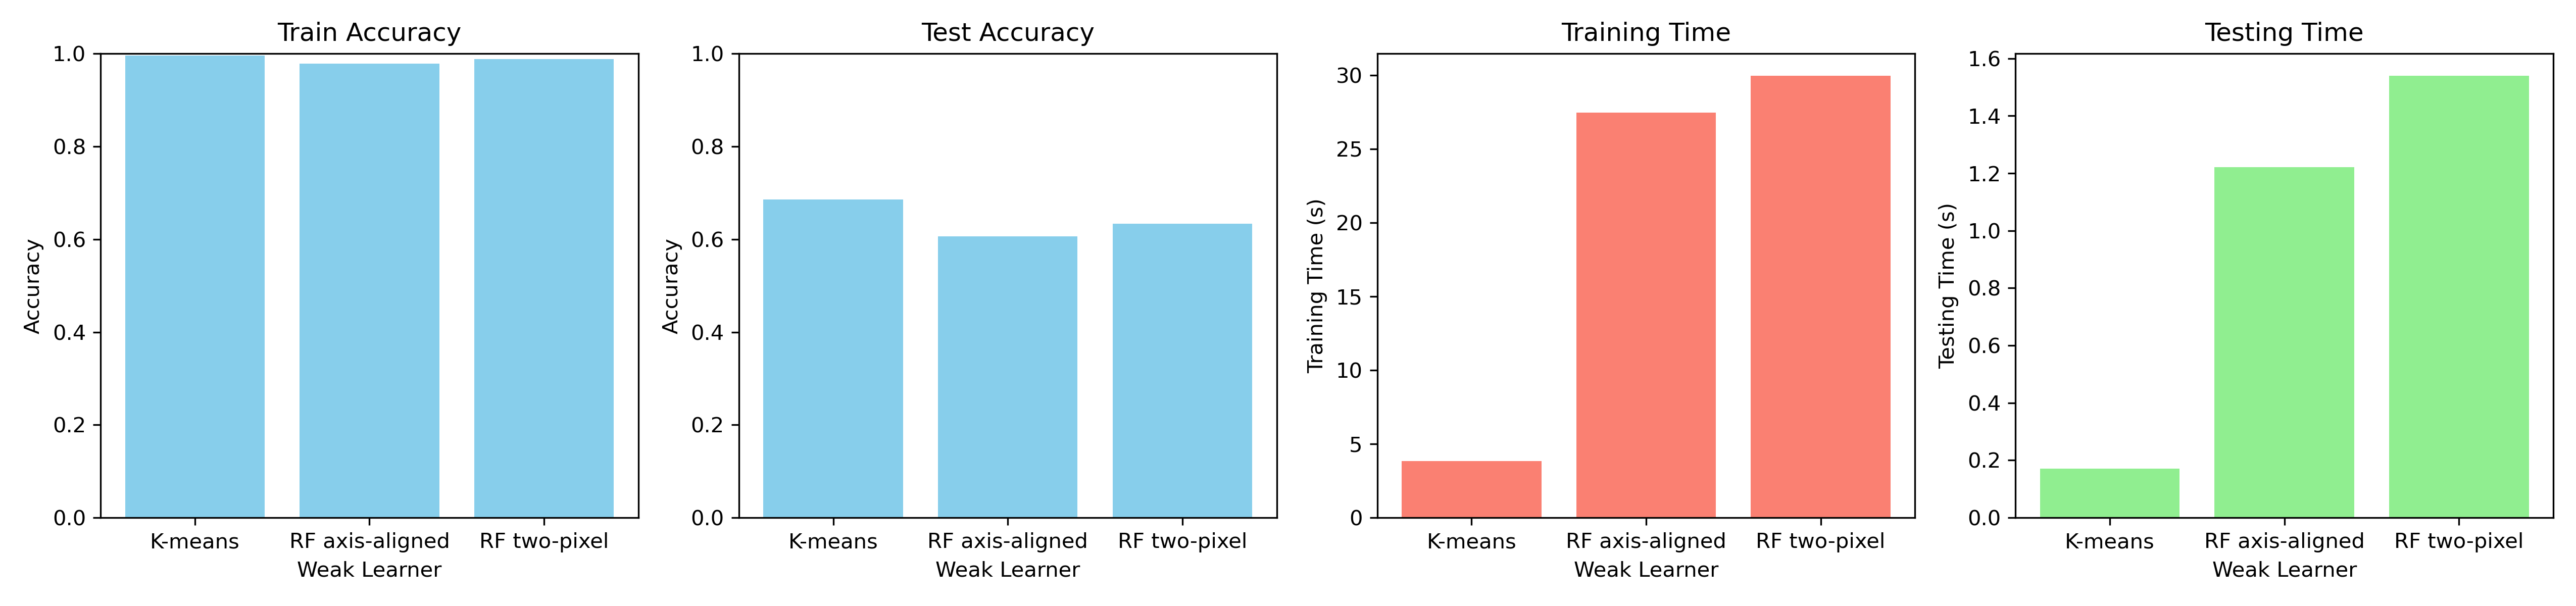
\includegraphics[width=0.8\linewidth]{image/q3-fig4.png}
	\caption{Comparison between different vocabulary method}
	\label{fig:q3-fig4}
\end{figure}

\begin{table}
	\centering
	\setlength{\tabcolsep}{6pt} % Adjust column spacing
	\renewcommand{\arraystretch}{1.5} % Adjust row height
	\resizebox{\linewidth}{!}{ % Scale table to fit text width
		\begin{tabular}{|c||c|c|c|c|}
			\hline
			& K-means,size=64 & K-means,size=256 & Random forest,size=64 & Random forest,size=256\\ \hline\hline
			Train Accuracy(\%) & 98.5 & 99.50 & 97.0 & 97.9 \\ \hline
			Inner-class cosine similarity & 0.735 & 0.708 & 0.863 & 0.844 \\ \hline
			Between-class cosine similarity & 0.564 & 0.577 & 0.743 & 0.711 \\ \hline
			Inner/Between & 1.303 & 1.227 & 1.161 & 1.187 \\ \hline
		\end{tabular}
	}
	\caption{Training data: K-means vs RF vocabulary}
	\label{table:q3-1}
\end{table}

\begin{table}
	\centering
	\setlength{\tabcolsep}{6pt} % Adjust column spacing
	\renewcommand{\arraystretch}{1.5} % Adjust row height
	\resizebox{\linewidth}{!}{ % Scale table to fit text width
		\begin{tabular}{|c||c|c|c|c|}
			\hline
			& K-means,size=64 & K-means,size=256 & Random forest,size=64 & Random forest,size=256\\ \hline\hline
			Test Accurac(\%) & 65.7 & 68.5 & 56.0 & 60.67 \\ \hline
			Inner-class cosine similarity & 0.710 & 0.698 & 0.856 & 0.833 \\ \hline
			Between-class cosine similarity & 0.572 & 0.592 & 0.766 & 0.728 \\ \hline
			Inner/Between & 1.240 & 1.179 & 1.117 & 1.143 \\ \hline
		\end{tabular}
	}
	\caption{Testing data: K-means vs RF vocabulary}
	\label{table:q3-2}
\end{table}


